



\section{Experiment 1}

In the literature of SA in Turkish, it is claimed that SA is only operational for inflectional suffixes \citep{orgun1995flat,kornfilt1996some,broadwell2008turkish, kornfilt2012revisiting} apart from \citet{akkucs2016suspended}. Isolated examples for SA of derivational suffixes can be found in corpora, but the literature treats them as exceptions. One similarity of this exceptionalism can be argued for the instances of SA in German. The examples provided in German \citep{pounder2006broken} have a dash "-" character at word endings where the suspended affix should be recovered, and the examples are from written literature sources dating back to 17$^{th}$ century. I designed a simple acceptability study to see whether SA of derivational suffixes are acceptable, and how the conjoiner choice affects the acceptability. I took a subset of the derivational suffixes that take nominal bases and produce nominals from a list in \citet{goksel2004turkish}. I give the derivation examples for the suffixes in (\ref{derivationalsuffixes}).  


\begin{exe}
  \begin{multicols}{2}
    \ex \label{derivationalsuffixes}
    \begin{xlist}
        \ex \gll düş-er-cesine \\ 
        fall-{\Aor}-{\Der} \\
        \glt `as if falling'
        
        \ex \gll yalan-cı \\ 
        lie-{\Der} \\ 
        \glt `liar'
        
        \ex \gll kahve-msi renk \\ 
        coffee-{\Der} colour \\
        \glt `colour resembling coffee'

        \ex \gll üç-üncü \\ 
        three-{\Der} \\
        \glt `third'

        \ex \gll sorun-lu adam \\ 
        problem-{\Der} man \\
        \glt `troubled man'
        
        \ex \gll düşman-lık \\ 
        enemy-{\Der} \\
        \glt `enmity'
        
        \ex \gll sınır-sız internet \\ 
        limit-{\Der} internet \\
        \glt `limitless internet'
        
        \ex \gll iki-şer \\ two-{\Der} \\
        \glt `two by two'
    \end{xlist}
    \end{multicols}
\end{exe}

The suffixes I chose do not have a particular property that makes them suitable candidates for SA. I used some of the observations of \citet{yoon2017lexical} where he suggests that some suffixes belong to a different morphological phase and retain their atomic properties even after vocabulary insertion. The morphemes that retain syntactic visibility choose category assigned bases and can take part in SA. Among the suffixes I selected, some show differences in what they take as a base. In (\ref{suffixesdiffer}), I provide a small description for the unique differences that some suffixes display.

\begin{exe}
\ex \label{suffixesdiffer}
\begin{itemize}
\item \textit{-CasInA} can take bases that are modified with a participle like {\Prf}, {\Prog}, or {\Aor}. 

\item \textit{-CI} takes noun bases and it is an agent nominalizer

\item \textit{-(I)msI} takes properties (adjectives,nouns) and returns properties similar but not equal to its base

\item \textit{-(I)ncI} takes numerals and returns an ordinal numeral

\item \textit{-(ş)Ar} takes numerals and returns adverbs

\end{itemize}
\end{exe}

I designed an acceptability study where a yes or no answer is provided for an expression hosting an SA construction. My purpose in this experiment was to investigate how much the suspension of the suffixes in (\ref{derivationalsuffixes}) were acceptable and how they compared to {\Acc}. Additionally, I investigated the effect of a conjoiner choice between \textit{ve} `and' and \textit{veya} `or'. In the following subsections I lay out the participants, materials, procedure, results, and analysis of the experiment.

\subsection{Participants}

The participants were 214 students from Boğaziçi University who are native speakers of Turkish. In exchange for their participation, they received 1 point to their overall course score with the consent of the course's instructor.


\subsection{Materials}

The experiment comprised of two variables: Suffix with 9 different levels (8 derivational and 1 inflectional {\Acc} suffixes) and Conjoiner with 2 levels (\textit{ve}`and', \textit{veya} `or'). For each suffix there were 3 distinct items. This way there were 54 experimental items. Additionally there were 27 grammatical and 27 ungrammatical fillers. A latin square design by conjoiner type was applied, forming two lists of 27. This resulted in each participant seeing only 27 experimental items and 54 fillers. The order of trials was randomized for each participant. An example set of experimental items for {\Acc} and \textit{-CAsInA} is given in (\ref{acceptabilityexe}). I carried out the experiment using ibexfarm \citep{drummond2013ibex}. For the full list of items and fillers (1-27 and 100-154), see Appendix \ref{acceptabilityitems}.

\begin{exe}
    \ex \label{acceptabilityexe}
    \begin{xlist}
    \ex {\Der}\_{\And} \\* 
    \gll Ev-e koş-ar ve zıpla-r-casına gel-di-m. \\ 
    house-{\Dat} run-{\Aor} {\And} jump-{\Aor}-{\Der} come-{\Pst}.{\Fsg} \\
    \glt ${}$
    
    \ex {\Der}\_{\Or} \\*
    \gll Ev-e koş-ar veya zıpla-r-casına gel-di-m. \\ 
    house-{\Dat} run-{\Aor} {\Or} jump-{\Aor}-{\Der} come-{\Pst}.{\Fsg} \\
    \glt `I came home as if running and/or jumping.' 
 
    \ex {\Infl}\_{\And} \\*
    \gll Ev-e defter ve kitab-ı getir-di-m. \\ 
    house-{\Dat} notebook {\And} book-{\Acc} bring-{\Pst}.{\Fsg} \\
    \glt ${}$
    
    \ex {\Infl}\_{\Or} \\*
    \gll Ev-e defter veya kitab-ı getir-di-m. \\ 
    house-{\Dat} notebook {\Or} book-{\Acc} bring-{\Pst}.{\Fsg} \\
    \glt `I brought home the book and/or the notebook.' 
    \end{xlist}
\end{exe}


\subsection{Procedure}

Participants were provided with a link to the experiment prompting them with a consent page. Upon giving consent participants went through 5 practice items and they were prompted again for the beginning of the experiment. Each trial proceeded with a full sentence and participants decided on whether the sentence they read was a natural/ok sentence in Turkish. They professed their decision by pushing `Q' key for `yes' and `P' key for `no' on the keyboard. The experiment only recorded choice and response time. Participants were redirected to a separate page where they provided their student information to be relayed to the course's professor for the extra credit after the experiment was done. This information is kept separate from the experiment results, keeping participant information and experimental data anonymous.

\subsection{Results}

The results were recorded onto a csv file and imported to R \citep{team2013r} for data cleaning, aggregation, and analysis. The data consisted of 17415 data points before cleaning. 1 experimental item with a typo and 1 experimental item with a possible ambiguity are excluded from the data. A further 3 filler items are excluded because they had particular configurations that lead to increased misparsing like garden path sentences. After this exclusion, accuracies of the participants are calculated relying on their answers for filler items. 9 participants with accuracies lower than 70\% are excluded from the data. Trials that were not between 2-20 seconds of response time are considered outliers and also excluded from the data. This cleaning process resulted in the loss of 14\% of the data. In Figure \ref{fig:suffixacceptability}, I give the average acceptability of each suffix by conjoiner type\footnote{from here on out all vertical errorbars indicate confidence intervals adjusted for within subject variation \citep{cousineau2017varieties}.}.

\begin{knitrout}
\definecolor{shadecolor}{rgb}{0.969, 0.969, 0.969}\color{fgcolor}\begin{figure}[hbt!]

{\centering 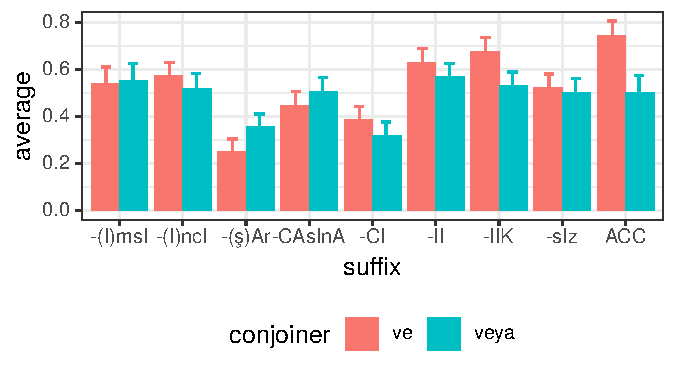
\includegraphics[]{experiments/acceptability/report/figure/suffixacceptability-1.pdf} 

}

\caption[First experiment, average acceptability for SA of suffixes by conjoiner]{First experiment, average acceptability for SA of suffixes by conjoiner}\label{fig:suffixacceptability}
\end{figure}


\end{knitrout}

For more inference in the acceptabilities, I fit a linear mixed model to responses using Conjoiner and Suffix as predictors with random effects for subject and item. I give the results of the model in Figure \ref{fig:derivationalmodel}. The points indicate median estimates and the thick line represents \%50 credible intervals and the thin line represents the \%95 credible intervals. The log-odd estimates above zero indicate increased odds of suspendability relative to the other derivational suffixes or conjoiner.

\begin{knitrout}
\definecolor{shadecolor}{rgb}{0.969, 0.969, 0.969}\color{fgcolor}\begin{figure}[hbt!]

{\centering 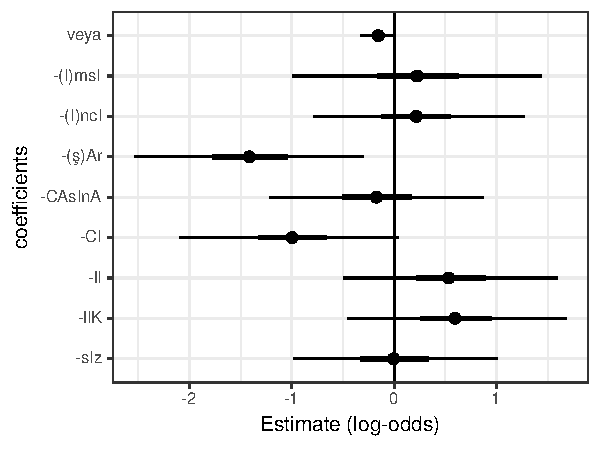
\includegraphics[]{experiments/acceptability/report/figure/derivationalmodel-1.pdf} 

}

\caption[First experiment, model results fit to grammaticality judgments with the predictors Suffix(8 derivational, 1 inflectional) and Conjoiner(ve, veya)]{First experiment, model results fit to grammaticality judgments with the predictors Suffix(8 derivational, 1 inflectional) and Conjoiner(ve, veya)}\label{fig:derivationalmodel}
\end{figure}


\end{knitrout}

\subsection{Analysis}

Figure \ref{fig:derivationalmodel} shows wide posterior probability distributions for the coefficients. One of the reasons for this is the low item count for each suffix. Another reason can be the varying degree of behaviour among the participants. The conjoiner choice of \textit{veya} "or" decreases the acceptability for SA in general. It also shows that suffixes do not behave uniformly in terms of acceptability. The suffixes \textit{-lI} and \textit{-lIK} seem to have the highest acceptabilities among all derivational suffixes, trailed by \textit{-(I)ncI} and \textit{-(I)msI}. There is no particular grouping of derivational suffixes in terms of acceptability. Positive estimates in this case don't indicate suspendability being grammatical or not, it is just a comparison made relative to a grand mean.

The two suffixes \textit{-(I)ncI} and \textit{-(ş)Ar} take numerals as their base and they both derive a nominal. They differ in average acceptability and the model results indicate a very small overlap in credible intervals. The suffix \textit{-CAsInA} takes participle forms as its base\footnote{it can take simple nouns too, but all the examples in the experiments are participle forms.} and  participle forms can end sentences with {\Tsg} interpretation in Turkish. This indicates that such bases are already assigned a lexical category. 

The varying degree of average acceptabilities among derivational suffixes and the similar results of the model show that SA of derivational suffixes in Turkish does not rely on a morphological phase analysis. If such an analysis were to hold true, the suffixes that take the same base should have behaved the same and the suffix taking participle base should have faired better. If a morphological phase analysis is not viable according to the experiment results, an approach that could capture the varying degree of acceptability is needed. The approach I take is the frequencies of the suffixes. For this purpose I extracted the frequencies of all four derivational suffixes (\textit{-lI,-lIK,-sIz}, and \textit{-CI} that TS Corpus \citep{sezer2013ts} had parsed). I give the relative proportion of the suffixes in Figure \ref{fig:suffixcorpus}. 

\begin{knitrout}
\definecolor{shadecolor}{rgb}{0.969, 0.969, 0.969}\color{fgcolor}\begin{figure}[hbt!]

{\centering 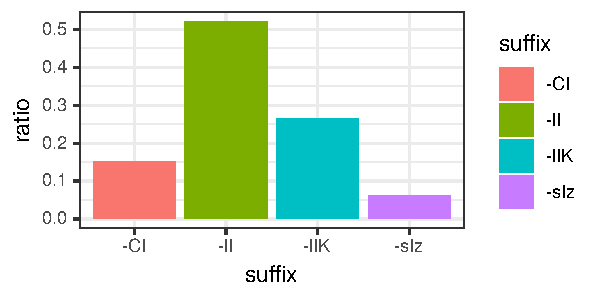
\includegraphics[]{experiments/acceptability/report/figure/suffixcorpus-1.pdf} 

}

\caption[Relative proportion of derivational suffixes in TS Corpus]{Relative proportion of derivational suffixes in TS Corpus}\label{fig:suffixcorpus}
\end{figure}


\end{knitrout}


The suffixes with the highest acceptabilities were \textit{-lI} and \textit{-lIK}. These two are the first two most frequent suffixes among the four presented in Figure \ref{fig:suffixcorpus}. Unfortunately not all derivational suffixes are readily extractable from the corpus data. The relative frequency of the suffixes in the corpus is not equally reflected by the experiment results and the experiment results indicate \textit{-CI} being less likely to be suspended compared to \textit{-sIz} even though it is relatively more frequent in the corpus.

The experiment results do not reflect the order of relative frequencies of these suffixes. The suffixes \textit{-lI} and \textit{-lIK} indeed have the highest acceptabilities in the experiment results, yet they aren't to the proportions of their relative frequencies. The suffix \textit{-CI} is relatively more frequent compared to \textit{-sIz} but fairs less acceptable in the experiment results. This means that raw frequency of a morpheme is not enough to explain the results. The two suffixes \textit{-(I)ncI} and \textit{-(I)msI} might hold an answer. These two suffixes receive similar acceptabilities with close estimates and overlapping credible intervals. 

I made a search in TS Corpus \citep{sezer2013ts} for examples of SA of the two suffixes \textit{-(I)ncI} and \textit{-(I)msI}. I provide two small CQP search keys \citep{hardie2012cqpweb}\footnote{CQP notation lets the user combine multiple features for a word in a corpus. These features include things like lexical category and morphological composition, together with regular expressions to specify certain character strings. A hit means a positive result matching the provided search key, and not all hits mean examples of suspended affixation.} in (\ref{tsinciquerry}) for SA of \textit{-(I)ncI}, with the numbers ranging from one to ten, and for \textit{-(I)msI} with noun and adjective bases.

\begin{exe}
\ex \label{tsinciquerry}
\begin{xlist}
\ex \label{inciquerry}\textit{-(I)ncI} TS corpus search key\\*
{[word="(bir{\textbar}iki{\textbar}üç{\textbar}dört{\textbar}beş{\textbar}altı{\textbar}yedi{\textbar}sekiz{\textbar}dokuz{\textbar}on)"][word="ve"]}
{[word="(.+nc(ı{\textbar}i{\textbar}u{\textbar}ü))"]}

\ex \textit{-(I)msI} TS corpus search key\\*
{[PosTag="Noun{\textbar}Adj"][word="ve"][PosTag="Adj" \& word="(.+ms(ı{\textbar}i{\textbar}u{\textbar}ü))"]}
\end{xlist}
\end{exe}

There are many examples for the SA of \textit{-(I)ncI} within $\sim$500 hits. The same can not be said for \textit{-(I)msI} which has the same acceptance rate as \textit{-(I)ncI} but the corpus search does not result in an SA of \textit{-(I)msI} within $\sim$500 hits. This discrepancy between similar acceptabilities but different corpus results can be explained by the relative frequency of these suffixes according to the context they are used in. The examples for SA of \textit{-(I)ncI} mostly comprise of texts written by clerks or reporters that refer to the passage or paragraph numbers of a law. In (\ref{corpusquerry}), I give some partial examples from the corpus search results for (\ref{inciquerry}). 

\begin{exe}
\ex SA of \textit{-(I)ncI} in corpus\\*
\label{corpusquerry}
\begin{xlist}

\ex \gll \ldots hüküm-ler bir ve iki-nci fıkra-lar-da yeniden düzenlendiğinden \ldots \\
\ldots provision-{\Pl} one {\And} two-{\Der} paragraph-{\Pl}-{\Loc} again change.because \ldots \\
\glt `\ldots because the provisions were adjusted again in the first and second paragraphs \ldots'

\ex \gll \ldots kanun-un dört ve beş-inci madde-ler-i değiş-tir-il-miş \ldots \\
\ldots law-{\Gen} four {\And} five-{\Der} article-{\Pl}-{\Poss}.{\Tsg} change-{\Caus}-{\Pass}-{\Prf}[{\Tsg}] \ldots \\
\glt`{\ldots} the forth and the fifth articles of the law were changed {\ldots}'

\end{xlist}
\end{exe}

There are examples in texts related to football, education, and others but texts related to law are more prominent. Unfortunately, text types are not tagged in TS Corpus. That's why it is hard to identify which text belongs to which context. I made a pseudo classification for the search results with the text categories of law, football, education, and others. I made the categorization depending on what the twenty words before and after the search hit contained. If those words contained an inflected or derived form of some words they are categorized according to the list of words they match. In (\ref{categorylist}), I provide what words defined a category of text. If twenty word periphery of the search hit contained an inflected or derived word outside the lists, it is categorized as `others'. This resulted in the classification of total 513 hits into 229 counts of law, 175 counts of others, 58 counts of education, and 51 counts of football in terms of what context the hit was in. This means that texts that are related to `law' are more numerous, thereby they are more likely to host examples for SA of \textit{-(I)ncI}.

\begin{exe}
\ex \label{categorylist}
\begin{xlist}
\ex Law: \textit{kanun, hüküm, fıkra, madde, paragraf, yönetmelik, nüsha}
\glt `law, provision, paragraph(archaic), article, paragraph, regulations, copy(archaic)'

\ex Football: \textit{gol, takım, lig, futbol, puan, oyun}
\glt `goal, team, football, point, game'

\ex Education: \textit{sınıf, ders, okul, eğitim, öğrenci}
\glt `class, course, school, education, student'

\end{xlist}
\end{exe}


\subsection{Conclusion}
The results of the experiment, comparisons of some derivational suffixes, and the related corpus searches provide two main observations about the suspendability of derivational suffixes. First, purely structural explanations can't predict varying acceptabilities. Second, suffixes with similar acceptabilities do not result in similar number of examples in the corpus. The examples in corpus show that the acceptability for SA of a derivational suffix is related to its relative frequency given the context it is used in. Taking these observations into consideration, I propose the following: The acceptability for SA of a derivational suffix is related to the relative frequency of the suffix given the context it is used in. When the relative frequency increases, the acceptability should increase too. Additionally the conjoiner \textit{veya} `or' decreases acceptability for all suffixes.











